\pdfoutput=1
\documentclass[aps,pra,reprint,superscriptaddress,nofootinbib,floatfix,
  showkeys]{revtex4-2}

\usepackage{amsmath,amssymb,bm}
\usepackage{booktabs}
\usepackage{graphicx}
\usepackage{microtype}
\usepackage{xcolor}
\usepackage[colorlinks=true,linkcolor=blue,citecolor=blue,urlcolor=blue]{hyperref}
\hypersetup{
  pdftitle={Variance-weighted measurement planning and rank-aware adaptive precision for quantum subspace eigensolvers},
  pdfauthor={Ginanjar Utama and Hermawan Kresno Dipojono},
  pdfsubject={Preregistered end-to-end study of weighted k-commuting grouping, paid-pilot Ritz replanning, rank-aware adaptive precision stopping, and noise-gated readout circuits}
}

\newcommand{\ket}[1]{\lvert #1\rangle}
\newcommand{\bra}[1]{\langle #1\rvert}
\newcommand{\avg}[1]{\langle #1\rangle}
\newcommand{\mHa}{\mathrm{mHa}}
\newcommand{\Ha}{\mathrm{Ha}}
\newcommand{\pkg}{\texttt{clifford\_qc}}
\newcommand{\Rhat}{\hat{R}}
\newcommand{\Remp}{R_{\mathrm{emp}}}
\newcommand{\CZmax}{\mathrm{CZ}_{\max}}
\newcommand{\tightcolumns}{\setlength{\tabcolsep}{3.5pt}}
\newcommand{\compactcolumns}{\setlength{\tabcolsep}{2.4pt}}
\renewcommand{\labelitemi}{\(\bullet\)}
\raggedbottom

% Auto-generated numeric macros derived from the frozen Commit 2 record.
% Auto-generated by paper_weighted_precision/make_tables.py. Do not edit.
\newcommand{\wpBehTwoRitzPilot}{19,992}
\newcommand{\wpBehTwoRitzRmse}{1.260}
\newcommand{\wpBiasRedMax}{13.4}
\newcommand{\wpBiasRedMin}{5.2}
\newcommand{\wpBootAnalysisReps}{2,000}
\newcommand{\wpBootAnalysisSeed}{2026112399}
\newcommand{\wpBootSolves}{49,696}
\newcommand{\wpDeclCommitFull}{73e48cc6f9fce7d0d0a568f5edf88ae441816423}
\newcommand{\wpDeclCommitShort}{73e48cc}
\newcommand{\wpExhausted}{4}
\newcommand{\wpFailed}{0}
\newcommand{\wpLihLdfFcLookTwoHi}{3.809}
\newcommand{\wpLihLdfFcLookTwoLo}{1.735}
\newcommand{\wpLihLdfFcLookTwoSE}{2.064}
\newcommand{\wpLihLdfFcLookZeroSE}{35.68}
\newcommand{\wpLihRitzFcRRatio}{1.628}
\newcommand{\wpLihSiFcLookTwoHi}{2.027}
\newcommand{\wpLihSiFcLookTwoLo}{1.958}
\newcommand{\wpLihSiFcLookTwoSE}{1.996}
\newcommand{\wpLihSiFcLookZeroSE}{13.88}
\newcommand{\wpLihSiFcRRatio}{1.397}
\newcommand{\wpLihSiQwcLookTwoSE}{1.539}
\newcommand{\wpLihSiQwcRRatio}{3.799}
\newcommand{\wpMeasuredSolves}{6,272}
\newcommand{\wpNoisyAnchorCount}{36}
\newcommand{\wpNumpyVer}{2.5.2}
\newcommand{\wpPartAAcq}{832}
\newcommand{\wpPartBAcq}{576}
\newcommand{\wpPilotShotsExact}{5,914,592}
\newcommand{\wpPoneaMedMax}{0.400}
\newcommand{\wpPoneaMedMin}{0.064}
\newcommand{\wpPoneaPassCount}{8}
\newcommand{\wpPoneaSpeedupMax}{13.6}
\newcommand{\wpPoneaSpeedupMin}{2.5}
\newcommand{\wpPoneaTotalCount}{9}
\newcommand{\wpPthreePassCount}{6}
\newcommand{\wpPthreeTotalCount}{6}
\newcommand{\wpPtwoHighTightBiasMax}{2.97}
\newcommand{\wpPtwoHighTightBiasMin}{1.17}
\newcommand{\wpPtwoHighUncBiasMax}{15.55}
\newcommand{\wpPtwoHighUncBiasMin}{13.82}
\newcommand{\wpPtwoLowTightFalseMax}{4}
\newcommand{\wpPtwoLowTightFalseMin}{1}
\newcommand{\wpPtwoLowUncFalseMax}{14}
\newcommand{\wpPtwoLowUncFalseMin}{13}
\newcommand{\wpPythonVer}{3.12.14}
\newcommand{\wpRRatioMax}{3.799}
\newcommand{\wpRRatioMin}{0.171}
\newcommand{\wpRmseRedMax}{7.1}
\newcommand{\wpRmseRedMin}{2.4}
\newcommand{\wpScFullBiasMax}{134.9}
\newcommand{\wpScFullBiasMin}{61.8}
\newcommand{\wpScipyVer}{1.18.0}
\newcommand{\wpSeedRoot}{2026112301}
\newcommand{\wpStretchedLdfQwcMeanM}{4.883}
\newcommand{\wpStretchedLdfRmse}{0.809}
\newcommand{\wpStretchedRitzRatioLdf}{0.820}
\newcommand{\wpStretchedRitzRmse}{0.467}
\newcommand{\wpStretchedRitzWidth}{2.68}
\newcommand{\wpStretchedSiKTwoMeanM}{3.418}
\newcommand{\wpStretchedSiKTwoSavePct}{30.0}
\newcommand{\wpStretchedSiKTwoVsSiQwcPct}{14.6}
\newcommand{\wpStretchedWords}{10,341}
\newcommand{\wpTargetMet}{1,404}
\newcommand{\wpTotalAcq}{1,408}
\newcommand{\wpTotalShotsB}{3.14}
\newcommand{\wpTotalShotsExact}{3,144,593,750}
\newcommand{\wpWidthBootRatioMax}{2.88}
\newcommand{\wpWidthBootRatioMin}{2.78}
\newcommand{\wpWidthExhErrMax}{0.694}
\newcommand{\wpWidthExhErrMin}{0.023}
\newcommand{\wpWidthMeanRatioMax}{5.78}
\newcommand{\wpWidthMeanRatioMin}{5.43}
\newcommand{\wpWidthRmseMax}{0.53}
\newcommand{\wpWidthRmseMin}{0.45}


\begin{document}

\title{Variance-weighted measurement planning and rank-aware adaptive precision for quantum subspace eigensolvers}

\author{Ginanjar Utama}
\email{ginanjar.utama@gmail.com}
\affiliation{Department of Engineering Physics, Institut Teknologi Bandung,
Bandung, Indonesia}

\author{Hermawan Kresno Dipojono}
\email{dipojono@itb.ac.id}
\affiliation{Department of Engineering Physics, Institut Teknologi Bandung,
Bandung, Indonesia}

\date{November 22, 2026}

\begin{abstract}
Quantum subspace eigensolvers estimate projected overlap and Hamiltonian
matrices from finite-shot Pauli expectations, yet measurement grouping and
adaptive stopping are usually evaluated in isolation: grouping studies count
commuting cliques while stopping studies fix qubit-wise-commuting (QWC)
readouts.  We present a preregistered, density-free workflow and end-to-end
evaluation that couples variance-weighted \(k\)-commuting sorted insertion,
paid-pilot Ritz-weighted replanning, and two-qubit noise-gated readout circuits
directly to a rank-aware adaptive precision controller.  All analysis scripts,
shot schedules, random-seed derivations, and primary pass/fail criteria
(P1a--P3) were frozen at commit \texttt{\wpDeclCommitShort} prior to drawing
any evaluation outcomes, then executed under a pinned software stack
(Python~\wpPythonVer, NumPy~\wpNumpyVer, SciPy~\wpScipyVer, single-threaded
BLAS) across \wpTotalAcq{} acquisitions totaling \wpTotalShotsB{}~billion
simulated physical shots (\wpMeasuredSolves{} measured solves, \wpBootSolves{}
bootstrap solves, \wpFailed{} numerical failures, and \wpExhausted{} schedule
exhaustions).  Under matched total physical-shot schedules on eight-qubit
BeH\(_2\), LiH, and H\(_4\) banks, bank-weighted sorted insertion passes
\wpPoneaPassCount{}/\wpPoneaTotalCount{} P1a cells with Holm--Bonferroni
significance, cutting mean shots by \wpPoneaSpeedupMin{}\(\times\) to
\wpPoneaSpeedupMax{}\(\times\) relative to unweighted largest-degree grouping
even on QWC where weighted grouping uses \emph{more} settings; the single
failing P1a cell is a discrete look-grid tie on LiH (\(k=8\)).  Paid-pilot
Ritz replanning reduces BeH\(_2\) shots a further \(2.5\times\), whereas on LiH
QWC beats both fully commuting (FC) arms by \(2.5\times\) because favorable
state-dependent covariance lifts \(\Remp/\Rhat\) to \wpLihSiQwcRRatio{}.  On a
stretched ten-qubit LiH bank (\wpStretchedWords{} Pauli words, rank~4
straddling the overlap cutoff), both \(k=2\) weighted arms pass P2 with
\(16/16\) true precision stops, \(0\) reduced-rank stops, and up to
\wpStretchedSiKTwoSavePct{}\% lower mean shots than unweighted QWC.  Under
gate-level two-qubit depolarizing noise, tight noise gating (\(\CZmax = 1\))
passes all \wpPthreePassCount{}/\wpPthreeTotalCount{} P3 cells, reducing
infinite-shot bias by \wpBiasRedMin{}\(\times\)--\wpBiasRedMax{}\(\times\) and
finite-shot RMSE by \wpRmseRedMin{}\(\times\)--\wpRmseRedMax{}\(\times\)
relative to unconstrained FC, whereas unmitigated readout bit-flip error
(\(p_{\mathrm{ro}}=0.02\)) induces \(+\wpScFullBiasMin{}\) to
\(+\wpScFullBiasMax{}\,\mHa\) bias across \emph{every} arm including QWC.
These are classical statevector and gate-level noise simulations on small
fixed molecular banks, not hardware demonstrations or quantum advantage claims.
\end{abstract}

\keywords{quantum subspace diagonalization, Pauli measurement grouping,
variance-weighted sorted insertion, adaptive shot allocation, rank-aware
stopping, noise-gated readout circuits}

\maketitle

\section{Introduction}
\label{sec:introduction}

Quantum subspace diagonalization (QSD), quantum subspace expansion (QSE), and
operator-generated subspace methods reconstruct a small generalized
eigenproblem \(H_{\mathrm{sub}} c = E S c\) from measured matrix elements on
one or more prepared states
\cite{mcclean2017qse,huggins2020nonorthogonal,stair2020krylov,utama2026operatorcentric,utama2026acase}.
Because finite-shot perturbations in \(S\) are amplified near its small
singular values \cite{epperly2022theory,lee2024sampling,zhang2024measurement},
practical accuracy depends simultaneously on \emph{two} layers that are usually
studied apart:
\begin{enumerate}
  \item \textbf{Measurement planning:} how the Pauli words required to assemble
    \(S\) and \(H_{\mathrm{sub}}\) are partitioned into commuting measurement
    settings, compiled into readout circuits, and bounded against two-qubit
    entangling-gate noise
    \cite{verteletskyi2020grouping,izmaylov2020unitary,crawford2021efficient,miller2024hardware,dalfavero2025kcommutativity,burns2024galic}.
  \item \textbf{Adaptive precision stopping:} how physical shots are allocated
    across settings over sequential looks, when the solver stops, and how
    overlap-rank instability or sampling uncertainty is guarded
    \cite{efron1979bootstrap,utama2026cliffordqc}.
\end{enumerate}

Evaluating these layers separately creates three well-known blind spots.
First, unweighted graph coloring heuristics such as largest-degree-first (LDF)
minimize the number of measurement settings \cite{verteletskyi2020grouping},
but setting count is a poor proxy for shot complexity when Hamiltonian and
overlap coefficients span orders of magnitude \cite{crawford2021efficient}.
Second, even when a partition improves the state-independent upper bound
\(\Rhat\), actual finite-shot variance depends on within-group covariances
\(\Remp\) on the prepared reference state, so fully commuting (FC) groupings
need not uniformly outperform qubit-wise commuting (QWC) groupings in physical
shots.  Third, unconstrained FC diagonalization circuits introduce multi-qubit
entangling gates whose depolarizing errors bias every measured matrix entry; an
adaptive stopping rule calibrated only for sampling variance will then declare
``target precision met'' around a strongly biased energy, turning variance
reduction into systematic false precision stops.

This short methods paper closes those three gaps in one preregistered,
end-to-end study built on the density-free workflow of \pkg{}
\cite{utama2026cliffordqc}.  Our contributions are fourfold:
\begin{itemize}
  \item We integrate variance-weighted \(k\)-commuting sorted insertion
    \cite{crawford2021efficient,dalfavero2025kcommutativity}, two-stage
    paid-pilot Ritz-weighted replanning, and GALIC-style per-setting two-qubit
    noise gating \cite{burns2024galic} atop a NumPy-only graph-state readout
    compiler directly inside the density-free rank-aware adaptive precision
    controller (\texttt{sampled\_precision}).
  \item We introduce a deterministic gate-level noisy readout simulator
    (\texttt{NoisyReadoutSimulator}) that applies explicit one-qubit,
    routing-inflated two-qubit, and readout bit-flip noise channels directly to
    compiled Clifford readout circuits and computes exact infinite-shot noisy
    projected energies \(E_\infty^{\mathrm{noisy}}\) for bias--variance
    decomposition.
  \item We execute a two-commit preregistered protocol: all scientific code,
    shot schedules, random seeds, bootstrap analysis settings, and primary
    criteria (P1a, P1b, P2, P3) were frozen at result-free commit
    \texttt{\wpDeclCommitShort} before drawing a single evaluation outcome,
    then executed across \wpTotalAcq{} acquisitions (\wpTotalShotsB{}~billion
    shots) and independently verified in continuous integration.
  \item We report every predeclared outcome transparently --- including one
    failed P1a cell caused by discrete look-grid quantization, one molecular
    bank where QWC beats FC by \(2.5\times\) via state-dependent covariance,
    four schedule exhaustions under opt-in bootstrap width gating, and the
    regime where unmitigated readout error dominates all groupings including
    QWC.
\end{itemize}

\section{Methods}
\label{sec:methods}

\subsection{Density-free graph-state measurement planning}
\label{sec:methods_planning}

Given a fixed single-reference generator bank \(\{A_i\}_{i=1}^{m}\) and qubit
Hamiltonian \(H = \sum_P h_P P\), the projected overlap and Hamiltonian
matrices have entries \(S_{ij} = \bra{\psi} A_i^\dagger A_j \ket{\psi}\) and
\(H_{ij} = \bra{\psi} A_i^\dagger H A_j \ket{\psi}\).  Expanding every product
in the Pauli basis yields a single shared word bank \(\mathcal{W}\) and linear
functionals \(\{f_{ij}^{(S)}, f_{ij}^{(H)}\}\) stored in packed coefficient
form \cite{utama2026cliffordqc}.  Crucially, no \(2^n \times 2^n\) density
matrix is ever formed by the consumer: the measurement planner and adaptive
controller interact with the reference solely through compiled measurement
settings and sampled bitstring histograms.

Each commuting group \(G_g \subseteq \mathcal{W}\) is constrained by
\(k\)-commutativity \cite{dalfavero2025kcommutativity}: the \(n\)-qubit
register is partitioned into blocks of size at most \(k\) (\(k=1\) gives QWC,
\(k=2\) restricts entangling readout circuits to disjoint qubit pairs of depth
at most~1, and \(k=n\) gives unconstrained FC).  Every group is compiled into a
Clifford readout circuit using the NumPy-only graph-state synthesizer
(\texttt{method="graph\_state"}), with each Pauli word assigned to exactly one
setting (\texttt{assigned} pooling).

\subsection{Variance-weighted sorted insertion and Ritz replanning}
\label{sec:methods_weighting}

To prioritize shot variance rather than clique count, we replace unweighted
largest-degree-first (LDF) coloring with weighted sorted insertion (SI)
\cite{crawford2021efficient}.  For a nonnegative word-weight map
\(w: \mathcal{W} \to \mathbb{R}_{\ge 0}\), words are ordered by descending
\(w(P)\) and inserted greedily into the first existing \(k\)-commuting group
compatible with every word already in that group.

We evaluate two density-free weight definitions:
\begin{enumerate}
  \item \textbf{Bank-weighted SI (\texttt{si\_*}):} uses only the static
    operator coefficients across the projected matrix functionals,
    \(w_{\mathrm{bank}}(P) = \sqrt{\sum_{\ell} |c_{\ell, P}|^2}\), requiring
    zero quantum shots.
  \item \textbf{Two-stage paid-pilot Ritz replanning (\texttt{ritz\_si\_*}):}
    first spends an independent pilot budget on a bank-weighted plan to
    estimate a preliminary Ritz eigenvector \(\hat{c}\) and weakest overlap
    eigenvector \(\hat{u}\), then computes first-order sensitivity weights
    combining the Ritz functional \(g_{\mathrm{Ritz}}(\hat{c})\) and normalized
    overlap-margin functional \(g_{\mathrm{ov}}(\hat{u})\) with mixing weight
    \(\lambda_{\mathrm{ov}} = 0.5\), replans the \(k\)-commuting partition
    once, and runs adaptive acquisition on the replanned settings.  To prevent
    cost hiding, every pilot shot is billed unconditionally to
    \texttt{total\_shots} and subtracted from the remaining look targets so
    single-stage and two-stage arms share the same cumulative physical-shot
    grid.
\end{enumerate}

For any linear functional \(F = \sum_P a_P P\) and partition \(\{G_g\}\),
optimal Neyman allocation gives a state-independent variance reduction factor
\(\Rhat\) (assuming unit single-word variance and zero off-diagonal covariance)
and a state-dependent covariance-aware factor \(\Remp\) computed from the
empirical within-group sample covariances \cite{crawford2021efficient}:
\begin{equation}
  \Rhat = \frac{\sum_P a_P^2}{\left(\sum_g \sqrt{\sum_{P \in G_g} a_P^2}\right)^2},
  \qquad
  \Remp = \frac{\sum_P \hat{\sigma}_P^2}{\left(\sum_g \hat{\sigma}_{G_g}\right)^2}.
  \label{eq:rhat_remp}
\end{equation}
Comparing \(\Remp/\Rhat\) exposes directly when state-dependent within-group
covariances help (\(\Remp > \Rhat\)) or hurt (\(\Remp < \Rhat\)) a grouping.

\subsection{GALIC-style two-qubit noise gating}
\label{sec:methods_galic}

Following the hardware-aware bias bound of GALIC \cite{burns2024galic}, our
\texttt{NoiseGatePolicy} enforces an explicit per-setting two-qubit gate cap
during greedy sorted insertion.  Given a native two-qubit depolarizing error
\(p_{2\mathrm{q}}\), routing overhead multiplier \(r_{\mathrm{route}}\), and
relative bias tolerance \(\varepsilon_{\mathrm{bias}}\), a candidate word
insertion into group \(G_g\) is accepted only if the compiled graph-state
readout circuit for \(G_g \cup \{P\}\) satisfies
\begin{equation}
  N_{\mathrm{CZ}}^{\mathrm{log}}(G_g \cup \{P\})
  \le \left\lfloor \frac{\ln(1 - \varepsilon_{\mathrm{bias}})}{r_{\mathrm{route}} \ln(1 - p_{2\mathrm{q}})} \right\rfloor.
  \label{eq:galic_cap}
\end{equation}
If no existing commuting group can absorb \(P\) within the cap, \(P\) opens a
new setting (always admissible with \(0\) two-qubit gates).  In our study, tight
gating (\(\varepsilon_{\mathrm{bias}} = 0.01\) at \(p_{2\mathrm{q}}=0.002\) or
\(0.05\) at \(p_{2\mathrm{q}}=0.010\), with \(r_{\mathrm{route}}=3\)) yields
\(\CZmax = 1\), while moderate gating yields \(\CZmax = 3\).

\subsection{Rank-aware adaptive precision stopping}
\label{sec:methods_stopping}

All arms are evaluated inside the unified raw-Ritz \texttt{sampled\_precision}
controller \cite{utama2026cliffordqc}.  At each predeclared look \(t \in
\{0,\dots,L-1\}\) along a matched total physical-shot schedule, the controller
assembles \((\hat{S}_t, \hat{H}_t)\), solves the thresholded generalized
eigenproblem with declared cutoff \(\tau_S\) and condition cap, estimates the
delta-method Ritz standard error \(\widehat{\mathrm{SE}}_t\), and evaluates
\texttt{RankStopPolicy(consecutive\_looks=2, margin\_delta=0.05)}.  The rank
guard differentiates the normalized extremal eigenvalues of
\(D^{-1/2} S D^{-1/2}\) (including the diagonal normalization derivative)
against the absolute cutoff \(\tau_S\), relative cutoff, and condition cap with
a three-comparison Bonferroni factor per look.  While the weakest lower margin
is nonpositive, the controller splits the next round budget between
margin-targeted overlap shots (half of the round if \(\widehat{\mathrm{SE}}_t >
\tau_{\mathrm{SE}}\), all of the round otherwise) and Ritz-variance-targeted
shots.  Stopping requires \(\widehat{\mathrm{SE}}_t \le 1.6\,\mHa\) and full
declared rank with positive lower margins on two consecutive looks.

We also test an opt-in bootstrap half-width guard (\texttt{si\_fc\_width}),
which additionally requires the \(L\)-look Bonferroni-adjusted percentile
bootstrap half-width \cite{efron1979bootstrap} to satisfy \(\le 1.6\,\mHa\)
before stopping.  All delta and bootstrap intervals are explicitly labeled
asymptotic/heuristic rather than finite-sample or anytime-valid certificates.

\subsection{Gate-level noisy readout simulator}
\label{sec:methods_noisy_sim}

To evaluate Part~B without circular assumptions, \texttt{NoisyReadoutSimulator}
propagates the exact prepared state \(\ket{\psi}\) through each compiled
readout circuit gate-by-gate using Kraus/channel evolution on the density
matrix: symmetric single-qubit depolarizing error \(p_{1\mathrm{q}}\) on each
1Q Clifford gate, two-qubit depolarizing error
\(p_{2\mathrm{q}}^{\mathrm{eff}} = 1 - (1 - p_{2\mathrm{q}})^{r_{\mathrm{route}}}\)
on each logical CZ gate, and independent symmetric computational-basis bit-flip
probability \(p_{\mathrm{ro}}\) before projective readout.  This yields both
exact finite-shot multinomial bitstring sampling and exact infinite-shot noisy
word expectations, hence exact \(E_\infty^{\mathrm{noisy}}\) and clean MSE
decomposition \(\mathrm{RMSE}^2 = \mathrm{Bias}^2 + \mathrm{Var}\) in every
cell.

\section{Preregistered Experimental Protocol}
\label{sec:protocol}

The complete protocol was frozen prior to evaluation in
\texttt{docs/restart/weighted\_precision\_declaration.json} at commit
\texttt{\wpDeclCommitFull} (Commit~1), binding the SHA-256 digests of every
tracked Python file under \texttt{clifford\_qc/} and \texttt{benchmarks/}, all
four FCIDUMP files \cite{knowles1989fcidump}, historical anchor records, and
the illustrative superconducting device card.  Development seed~\texttt{501}
was used solely to verify bank anchors and calibrate shot schedules prior to
freezing and is excluded from evaluation; evaluation seeds derive
deterministically from \texttt{seed\_root = \wpSeedRoot} via NumPy
\texttt{SeedSequence} with zero collisions across all \(2{,}928\) streams.

\begin{table*}[t]
\centering
\caption{Molecular test banks, exact projected energy targets, overlap-spectrum
conditioning (\(\lambda_{\min}/\tau_S\)), Pauli word counts, and static
Part~A compiled \texttt{graph\_state} plan metrics.  All numbers are generated
from the committed Commit~2 record.}
\label{tab:protocol_banks}
\tightcolumns
\begin{tabular}{l r l r l r r r r}
\toprule
Bank & Words & Rank (\(\lambda_{\min} / \tau_S\)) & Exact \(E\) (Ha) & Arm & Settings & \(\Rhat\) & \(\mathrm{CZ}_{\mathrm{tot}}\) (\(\CZmax\)) & \(d_{2\mathrm{q},\max}\) \\
\midrule
% Auto-generated by paper_weighted_precision/make_tables.py. Do not edit.
BeH$_2$ (8q) & $1,223$ & $3$ ($0.2106$; $0.005$) & $-15.560867$ & \texttt{ldf\_qwc} & $281$ & $2.15$ & $0$ ($0$) & $0$ \\
 &  &  &  & \texttt{si\_qwc} & $312$ & $3.78$ & $0$ ($0$) & $0$ \\
 &  &  &  & \texttt{ldf\_k2} & $37$ & $6.45$ & $108$ ($4$) & $1$ \\
 &  &  &  & \texttt{si\_k2} & $44$ & $14.13$ & $127$ ($4$) & $1$ \\
 &  &  &  & \texttt{ldf\_fc} & $12$ & $9.88$ & $71$ ($7$) & $5$ \\
 &  &  &  & \texttt{si\_fc} & $14$ & $18.11$ & $65$ ($7$) & $5$ \\
\midrule
LiH (8q) & $3,167$ & $3$ ($0.2106$; $0.005$) & $-7.863048$ & \texttt{ldf\_qwc} & $669$ & $2.09$ & $0$ ($0$) & $0$ \\
 &  &  &  & \texttt{si\_qwc} & $768$ & $7.28$ & $0$ ($0$) & $0$ \\
 &  &  &  & \texttt{ldf\_k2} & $278$ & $3.41$ & $517$ ($4$) & $1$ \\
 &  &  &  & \texttt{si\_k2} & $298$ & $19.49$ & $569$ ($4$) & $1$ \\
 &  &  &  & \texttt{ldf\_fc} & $61$ & $16.54$ & $343$ ($11$) & $6$ \\
 &  &  &  & \texttt{si\_fc} & $59$ & $26.07$ & $342$ ($12$) & $6$ \\
\midrule
H$_4$ (8q) & $3,051$ & $3$ ($0.2106$; $0.005$) & $-2.147929$ & \texttt{ldf\_qwc} & $701$ & $2.84$ & $0$ ($0$) & $0$ \\
 &  &  &  & \texttt{si\_qwc} & $794$ & $6.67$ & $0$ ($0$) & $0$ \\
 &  &  &  & \texttt{ldf\_k2} & $356$ & $4.32$ & $576$ ($4$) & $1$ \\
 &  &  &  & \texttt{si\_k2} & $399$ & $11.54$ & $598$ ($4$) & $1$ \\
 &  &  &  & \texttt{ldf\_fc} & $69$ & $16.29$ & $651$ ($18$) & $7$ \\
 &  &  &  & \texttt{si\_fc} & $61$ & $28.86$ & $432$ ($16$) & $7$ \\
\midrule
LiH (10q, str.) & $10,341$ & $4$ ($0.1042$; $0.104$) & $-7.763633$ & \texttt{ldf\_qwc} & $1,679$ & $2.92$ & $0$ ($0$) & $0$ \\
 &  &  &  & \texttt{si\_qwc} & $1,938$ & $8.27$ & $0$ ($0$) & $0$ \\
 &  &  &  & \texttt{si\_k2} & $490$ & $22.76$ & $1,294$ ($5$) & $1$ \\

\bottomrule
\end{tabular}
\end{table*}

Table~\ref{tab:protocol_banks} summarizes the four molecular banks and their
static compiled plans:
\begin{itemize}
  \item \textbf{Part~A (ideal shots, \wpPartAAcq{} acquisitions):} Three
    well-conditioned eight-qubit banks --- BeH\(_2\) (1,223 words), LiH (3,167
    words), and H\(_4\) (3,051 words), each rank~3 with \(\lambda_{\min} =
    0.2106 \gg \tau_S = 0.005\) --- tested across 8 arms
    (\texttt{ldf\_qwc}, \texttt{si\_qwc}, \texttt{ldf\_k2}, \texttt{si\_k2},
    \texttt{ldf\_fc}, \texttt{si\_fc}, \texttt{ritz\_si\_fc},
    \texttt{si\_fc\_width}), 32 outer replicas, 32 bootstrap replicates, and a
    six-look matched cumulative schedule (\([0.04, 0.10, 0.25, 0.625, 1.5625,
    3.90625]\times 10^6\) shots for BeH\(_2\)/LiH; up to \(9.766\times 10^6\)
    for H\(_4\)); plus the engineered near-cutoff ten-qubit stretched LiH bank
    (\wpStretchedWords{} words, rank~4 with \(\lambda_{\min} = 0.10417\)
    straddling \(\tau_S = 0.104\)) across 4 arms (\texttt{ldf\_qwc},
    \texttt{si\_qwc}, \texttt{si\_k2}, \texttt{ritz\_si\_k2}) and 16 outer
    replicas.
  \item \textbf{Part~B (gate-level noisy readout, \wpPartBAcq{} acquisitions):}
    BeH\(_2\), LiH, and H\(_4\) (16 outer replicas each) across 4 arms
    (\texttt{si\_qwc}, \texttt{si\_fc\_unconstrained},
    \texttt{si\_fc\_galic\_tight}, \texttt{si\_fc\_galic\_moderate}) under
    three noise regimes: (i)~\texttt{depol2q\_p002\_r3} (\(p_{2\mathrm{q}} =
    0.002, r_{\mathrm{route}} = 3, p_{1\mathrm{q}}=p_{\mathrm{ro}}=0\));
    (ii)~\texttt{depol2q\_p010\_r3} (\(p_{2\mathrm{q}} = 0.010,
    r_{\mathrm{route}} = 3\)); and (iii)~\texttt{sc\_card\_full}
    (\(p_{1\mathrm{q}} = 0.001, p_{2\mathrm{q}} = 0.010, r_{\mathrm{route}} =
    3, p_{\mathrm{ro}} = 0.02\)).
\end{itemize}

Four primary endpoints were frozen in \texttt{check\_weighted\_precision.py}
prior to execution:
\begin{itemize}
  \item \textbf{P1a:} On the nine eight-qubit matched-\(k\) pairs
    (\(k \in \{1,2,8\}\)), weighted SI passes a cell if median shot ratio
    \(\le 0.80\) (or strictly lower mean ratio on a median tie), \(\ge 30/32\)
    \texttt{target\_met} stops, \(0\) reduced-rank stops, and non-rejected
    unconditional 95\% bootstrap coverage (exact one-sided binomial lower tail
    \(p_{\mathrm{lo}} \ge 0.05/9\)); mean shot ratios are additionally tested
    with \wpBootAnalysisReps{}-resample percentile bootstrap CIs (seed
    \texttt{\wpBootAnalysisSeed}) and Holm--Bonferroni step-down
    \cite{holm1979simple}.
  \item \textbf{P1b (descriptive):} Report paired shot ratios, RMSE, 95\%
    coverage, and median \(\Remp/\Rhat\) for paid-pilot \texttt{ritz\_si\_fc}
    versus \texttt{si\_fc} and \texttt{si\_qwc} (and \texttt{si\_fc} versus
    \texttt{si\_qwc}) without forcing FC to beat QWC.
  \item \textbf{P2:} On stretched ten-qubit LiH, both \texttt{si\_k2} and
    \texttt{ritz\_si\_k2} must achieve \(\ge 12/16\) true precision stops
    (\texttt{target\_met} and \(|E - E_{\mathrm{exact}}| \le 1.6\,\mHa\)),
    \(\le 1/16\) false precision stops, and \(0\) reduced-rank stops.
  \item \textbf{P3:} Under both pure-2Q noise regimes across all three
    eight-qubit banks (6 cells), \texttt{si\_fc\_galic\_tight} must achieve
    strictly smaller exact \(|E_\infty^{\mathrm{noisy}} - E_{\mathrm{exact}}|\)
    and finite-shot RMSE than \texttt{si\_fc\_unconstrained}, and strictly
    fewer false stops whenever unconstrained FC has \(|\mathrm{bias}| >
    1.6\,\mHa\); \texttt{sc\_card\_full} is reported separately as a full-noise
    diagnostic.
\end{itemize}
Strict unconditional coverage counts \emph{only} eligible \texttt{target\_met}
stops in the numerator over all declared attempts in the denominator
(exhaustions and failures count as uncovered), with Wilson intervals
\cite{wilson1927probable} and stop-conditional coverage reported separately.

\section{Results}
\label{sec:results}

Execution at commit \texttt{\wpDeclCommitShort} produced
\texttt{docs/restart/weighted\_precision\_results.json.gz} containing all
\wpTotalAcq{} acquisitions, \wpTotalShotsExact{} simulated physical shots
(including \wpPilotShotsExact{} paid pilot shots), \wpMeasuredSolves{} measured
solves, and \wpBootSolves{} bootstrap solves.  Zero acquisitions or bootstraps
failed (\wpFailed{}/\wpTotalAcq{}); \wpTargetMet{}/\wpTotalAcq{} met their stop
guards and \wpExhausted{}/\wpTotalAcq{} exhausted their schedule (all four in
the opt-in \texttt{beh2\_8q} \texttt{si\_fc\_width} arm).  The independent
checker verified every row, all four occupation-space anchors, all
\wpNoisyAnchorCount{} independent infinite-shot noisy anchors, three full spot
replays, and Git commit chronology.

\subsection{P1a: Weighted SI versus unweighted LDF and setting-count paradox}
\label{sec:results_p1a}

\begin{figure*}[t]
  \centering
  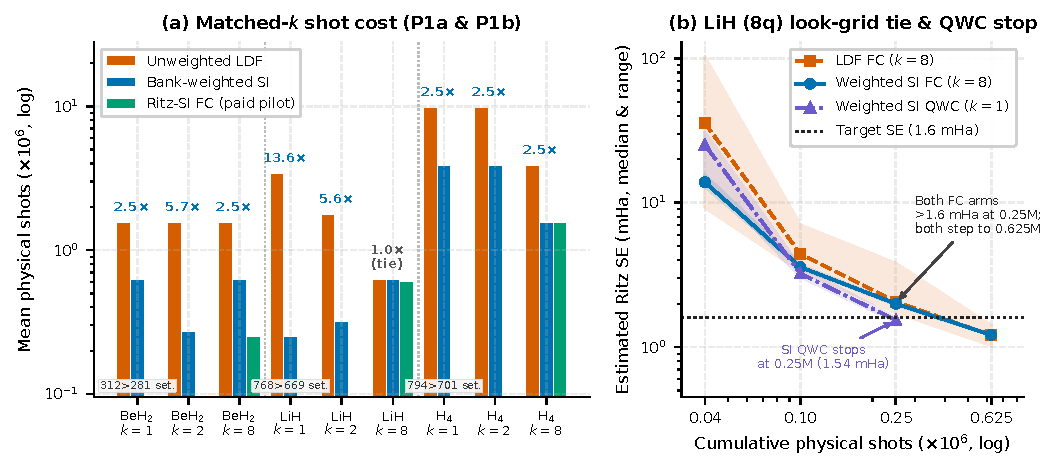
\includegraphics[width=\textwidth]{paper_assets/fig1_shot_savings_and_grid.pdf}
  \caption{(a)~Mean total physical shots across all nine predeclared P1a pairs
  (\(k \in \{1,2,8\}\)) plus paid-pilot Ritz-SI FC on the three eight-qubit
  molecular banks.  Speedup labels above each pair report unweighted LDF
  divided by weighted SI; gray badges at the bottom of the \(k=1\) pairs note
  that weighted SI uses \emph{more} QWC settings than LDF yet requires
  \(2.5\times\)--\wpPoneaSpeedupMax{}\(\times\) fewer shots.  (b)~Look-by-look
  median estimated Ritz SE (with min--max envelope over 32 replicas) on
  LiH~(8q), showing why both FC arms tie at \(0.625\times 10^6\) shots while
  weighted SI QWC stops early at \(0.25\times 10^6\).}
  \label{fig:shot_savings}
\end{figure*}

\begin{table*}[t]
\centering
\caption{Predeclared P1a matched-\(k\) hypothesis verdicts (Panel~A) and P1b
descriptive comparisons (Panel~B).  Shot ratios and 95\% confidence intervals
use \wpBootAnalysisReps{} bootstrap resamples (seed
\texttt{\wpBootAnalysisSeed}); Panel~A applies Holm--Bonferroni step-down to
\(p_{\mathrm{mean}\ge 1}\) and Bonferroni \(\alpha=0.05/9\) to unconditional
95\% bootstrap coverage \(p_{\mathrm{lo}}\).}
\label{tab:p1_verdicts}
\tightcolumns
\begin{tabular}{l c l c c c c l}
\toprule
Molecule & \(k\) & Pair (treat.\ / comp.) & Median ratio (95\% CI) & Mean ratio (95\% CI) & \(p_{\mathrm{mean}\ge 1}\) (Holm) / RMSE & 95\% boot (\(p_{\mathrm{lo}}\)) & Verdict / \(R/\Rhat\) \\
\midrule
% Auto-generated by paper_weighted_precision/make_tables.py. Do not edit.
\multicolumn{8}{l}{\textit{Panel A: Predeclared P1a --- Weighted SI vs.\ unweighted LDF at matched $k$}} \\
\midrule
BeH$_2$ (8q) & $1$ & \texttt{si\_qwc} / \texttt{ldf\_qwc} & $0.400$ $[0.400, 0.400]$ & $0.400$ $[0.400, 0.400]$ & $0.0000$ (Yes) & $32/32$ ($1.000$) & \textbf{PASS} \\
BeH$_2$ (8q) & $2$ & \texttt{si\_k2} / \texttt{ldf\_k2} & $0.160$ $[0.160, 0.160]$ & $0.175$ $[0.160, 0.198]$ & $0.0000$ (Yes) & $32/32$ ($1.000$) & \textbf{PASS} \\
BeH$_2$ (8q) & $8$ & \texttt{si\_fc} / \texttt{ldf\_fc} & $0.400$ $[0.400, 0.400]$ & $0.400$ $[0.400, 0.400]$ & $0.0000$ (Yes) & $31/32$ ($0.806$) & \textbf{PASS} \\
LiH (8q) & $1$ & \texttt{si\_qwc} / \texttt{ldf\_qwc} & $0.064$ $[0.064, 0.064]$ & $0.074$ $[0.068, 0.083]$ & $0.0000$ (Yes) & $31/32$ ($0.806$) & \textbf{PASS} \\
LiH (8q) & $2$ & \texttt{si\_k2} / \texttt{ldf\_k2} & $0.160$ $[0.160, 0.160]$ & $0.180$ $[0.147, 0.217]$ & $0.0000$ (Yes) & $32/32$ ($1.000$) & \textbf{PASS} \\
LiH (8q) & $8$ & \texttt{si\_fc} / \texttt{ldf\_fc} & $1.000$ $[1.000, 1.000]$ & $1.000$ $[1.000, 1.000]$ & $1.0000$ (No) & $32/32$ ($1.000$) & \textbf{FAIL} (tie) \\
H$_4$ (8q) & $1$ & \texttt{si\_qwc} / \texttt{ldf\_qwc} & $0.400$ $[0.400, 0.400]$ & $0.400$ $[0.400, 0.400]$ & $0.0000$ (Yes) & $32/32$ ($1.000$) & \textbf{PASS} \\
H$_4$ (8q) & $2$ & \texttt{si\_k2} / \texttt{ldf\_k2} & $0.400$ $[0.400, 0.400]$ & $0.400$ $[0.400, 0.400]$ & $0.0000$ (Yes) & $30/32$ ($0.480$) & \textbf{PASS} \\
H$_4$ (8q) & $8$ & \texttt{si\_fc} / \texttt{ldf\_fc} & $0.400$ $[0.400, 0.400]$ & $0.400$ $[0.400, 0.400]$ & $0.0000$ (Yes) & $32/32$ ($1.000$) & \textbf{PASS} \\
\midrule
\multicolumn{8}{l}{\textit{Panel B: Predeclared P1b (descriptive) --- Paid-pilot Ritz replanning vs.\ bank-weighted FC and QWC}} \\
\midrule
BeH$_2$ (8q) & --- & \texttt{ritz\_si\_fc} / \texttt{si\_fc} & $0.400$ $[0.400, 0.400]$ & $0.400$ $[0.400, 0.400]$ & RMSE $1.260$ & $32/32$ & $R/\hat{R} = 0.348$ \\
BeH$_2$ (8q) & --- & \texttt{ritz\_si\_fc} / \texttt{si\_qwc} & $0.400$ $[0.400, 0.400]$ & $0.400$ $[0.400, 0.400]$ & RMSE $1.260$ & $32/32$ & $R/\hat{R} = 0.348$ \\
BeH$_2$ (8q) & --- & \texttt{si\_fc} / \texttt{si\_qwc} & $1.000$ $[1.000, 1.000]$ & $1.000$ $[1.000, 1.000]$ & RMSE $1.319$ & $31/32$ & $R/\hat{R} = 0.209$ \\
LiH (8q) & --- & \texttt{ritz\_si\_fc} / \texttt{si\_fc} & $1.000$ $[1.000, 1.000]$ & $0.963$ $[0.906, 1.000]$ & RMSE $1.189$ & $32/32$ & $R/\hat{R} = 1.628$ \\
LiH (8q) & --- & \texttt{ritz\_si\_fc} / \texttt{si\_qwc} & $2.500$ $[2.500, 2.500]$ & $2.406$ $[2.266, 2.500]$ & RMSE $1.189$ & $32/32$ & $R/\hat{R} = 1.628$ \\
LiH (8q) & --- & \texttt{si\_fc} / \texttt{si\_qwc} & $2.500$ $[2.500, 2.500]$ & $2.500$ $[2.500, 2.500]$ & RMSE $1.113$ & $32/32$ & $R/\hat{R} = 1.397$ \\
H$_4$ (8q) & --- & \texttt{ritz\_si\_fc} / \texttt{si\_fc} & $1.000$ $[1.000, 1.000]$ & $1.000$ $[1.000, 1.000]$ & RMSE $1.133$ & $32/32$ & $R/\hat{R} = 0.547$ \\
H$_4$ (8q) & --- & \texttt{ritz\_si\_fc} / \texttt{si\_qwc} & $0.400$ $[0.400, 0.400]$ & $0.400$ $[0.400, 0.400]$ & RMSE $1.133$ & $32/32$ & $R/\hat{R} = 0.547$ \\
H$_4$ (8q) & --- & \texttt{si\_fc} / \texttt{si\_qwc} & $0.400$ $[0.400, 0.400]$ & $0.400$ $[0.400, 0.400]$ & RMSE $1.088$ & $32/32$ & $R/\hat{R} = 0.512$ \\

\bottomrule
\end{tabular}
\end{table*}

Weighted sorted insertion passes \wpPoneaPassCount{}/\wpPoneaTotalCount{} P1a
cells (Table~\ref{tab:p1_verdicts}, Panel~A; Fig.~\ref{fig:shot_savings}(a)).
Every passing cell is Holm--Bonferroni significant (\(p_{\mathrm{mean}\ge 1} =
0.0000\)), reduces median shots to \wpPoneaMedMin{}\(\times\)--\wpPoneaMedMax{}\(\times\)
(\wpPoneaSpeedupMin{}\(\times\)--\wpPoneaSpeedupMax{}\(\times\) fewer mean
shots), achieves \(32/32\) \texttt{target\_met} stops with \(0\) reduced-rank
stops, and maintains \(30/32\)--\(32/32\) unconditional 95\% bootstrap
coverage.

The QWC (\(k=1\)) cells directly refute setting count as a proxy for adaptive
measurement cost: bank-weighted \texttt{si\_qwc} produces \emph{more} commuting
settings than \texttt{ldf\_qwc} on every molecule (\(312 > 281\) on BeH\(_2\),
\(768 > 669\) on LiH, \(794 > 701\) on H\(_4\); Table~\ref{tab:protocol_banks}),
yet cuts mean physical shots by \(2.5\times\), \wpPoneaSpeedupMax{}\(\times\),
and \(2.5\times\), respectively, because keeping high-weight Hamiltonian terms
together lowers the Neyman-allocated variance factor \(\Rhat\) by
\(1.8\times\)--\(3.5\times\).

Because P1a requires all nine cells to pass, the conjunction evaluates to
\texttt{all\_passed = false} due to one discrete look-grid tie on LiH~(8q) at
\(k=8\) (\texttt{si\_fc} vs.\ \texttt{ldf\_fc}, ratio \(1.000\)).
Figure~\ref{fig:shot_savings}(b) shows the underlying trajectory: at look~0
(\(0.04\times 10^6\) shots), \texttt{si\_fc} already reduces median SE by
\(2.6\times\) (\wpLihSiFcLookZeroSE{} vs.\ \wpLihLdfFcLookZeroSE{}\,\(\mHa\)),
and at look~2 (\(0.25\times 10^6\) shots) \texttt{si\_fc} exhibits lower and
far tighter SE (\wpLihSiFcLookTwoSE{}\,\(\mHa\), range
[\wpLihSiFcLookTwoLo{}, \wpLihSiFcLookTwoHi{}]) than \texttt{ldf\_fc}
(\wpLihLdfFcLookTwoSE{}\,\(\mHa\), range [\wpLihLdfFcLookTwoLo{},
\wpLihLdfFcLookTwoHi{}]).  Because both lie slightly above the \(1.6\,\mHa\)
stop threshold, the \(2.5\times\) geometric look spacing quantizes all 32
replicas of both arms onto \(0.625\times 10^6\) shots.

\subsection{P1b: Paid-pilot Ritz replanning and covariance reversal}
\label{sec:results_p1b}

\begin{figure*}[t]
  \centering
  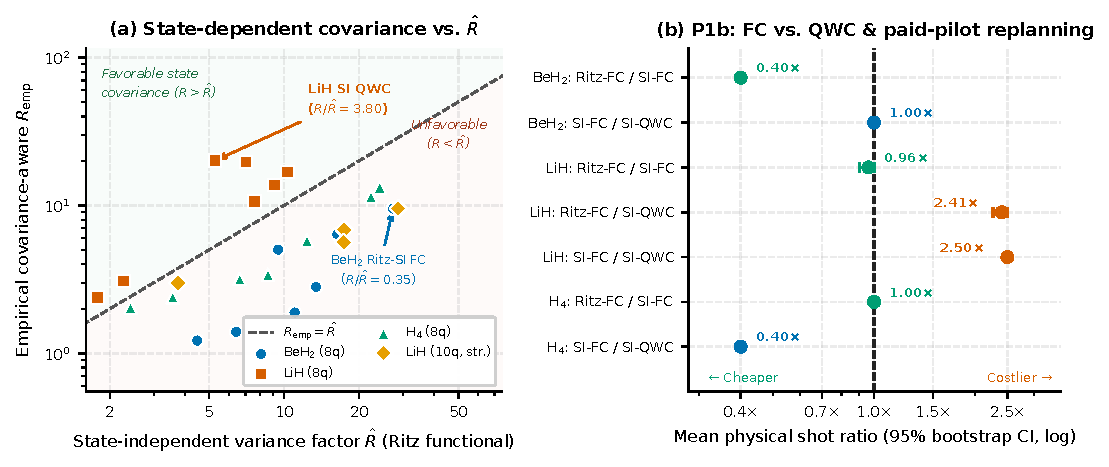
\includegraphics[width=\textwidth]{paper_assets/fig2_r_emp_vs_r_hat.pdf}
  \caption{(a)~Empirical covariance-aware variance factor \(\Remp\) versus
  state-independent \(\Rhat\) across all Part~A arms (excluding width-guarded
  duplicates).  Points above the dashed diagonal benefit from favorable
  within-group covariances on the prepared state; points below suffer
  unfavorable positive covariances.  (b)~Mean physical-shot ratios (with 95\%
  bootstrap CIs) for the predeclared P1b comparisons, showing how state
  covariance reverses FC vs.\ QWC across molecules.}
  \label{fig:r_emp_vs_r_hat}
\end{figure*}

Table~\ref{tab:p1_verdicts} (Panel~B) and Fig.~\ref{fig:r_emp_vs_r_hat} show
two distinct effects across molecules:
\begin{enumerate}
  \item \textbf{Paid-pilot Ritz replanning helps most when static bank weights
    misalign with the Ritz vector.}  On BeH\(_2\)~(8q), \texttt{ritz\_si\_fc}
    (including its \wpBehTwoRitzPilot{}-shot pilot) cuts total physical shots
    by \(2.5\times\) below \emph{both} \texttt{si\_fc} and \texttt{si\_qwc}
    (\(0.250\times 10^6\) vs.\ \(0.625\times 10^6\), \(32/32\) 95\% coverage,
    RMSE \wpBehTwoRitzRmse{}\,\(\mHa\)).  On LiH~(8q), it trims mean shots
    modestly versus \texttt{si\_fc} (\(0.963\times\)), and on H\(_4\)~(8q) it
    matches \texttt{si\_fc} (\(1.000\times\)).
  \item \textbf{FC does not uniformly beat QWC.}  While FC cuts shots by
    \(2.5\times\) relative to \texttt{si\_qwc} on H\(_4\)~(8q), \emph{both} FC
    arms are \(2.5\times\) more expensive than \texttt{si\_qwc} on LiH~(8q)
    (\(0.625\times 10^6\) / \(0.602\times 10^6\) vs.\ \(0.250\times 10^6\)).
    Figure~\ref{fig:r_emp_vs_r_hat}(a) resolves the mechanism: across all 28
    Part~A cells, \(\Remp/\Rhat\) spans \wpRRatioMin{} to \wpRRatioMax{}.  On
    LiH~(8q), \texttt{si\_qwc} achieves \(\Remp/\Rhat = \wpLihSiQwcRRatio{}\)
    (allowing look-2 SE \wpLihSiQwcLookTwoSE{}\,\(\mHa \le 1.6\,\mHa\)),
    substantially outperforming \texttt{si\_fc} (\wpLihSiFcRRatio{}) and
    \texttt{ritz\_si\_fc} (\wpLihRitzFcRRatio{}).  Reporting state-independent
    \(\Rhat\) without empirical \(\Remp\) would have predicted the opposite
    ordering.
\end{enumerate}

\subsection{P2: Stretched ten-qubit rank transfer and width-guard cost}
\label{sec:results_p2}

\begin{figure*}[t]
  \centering
  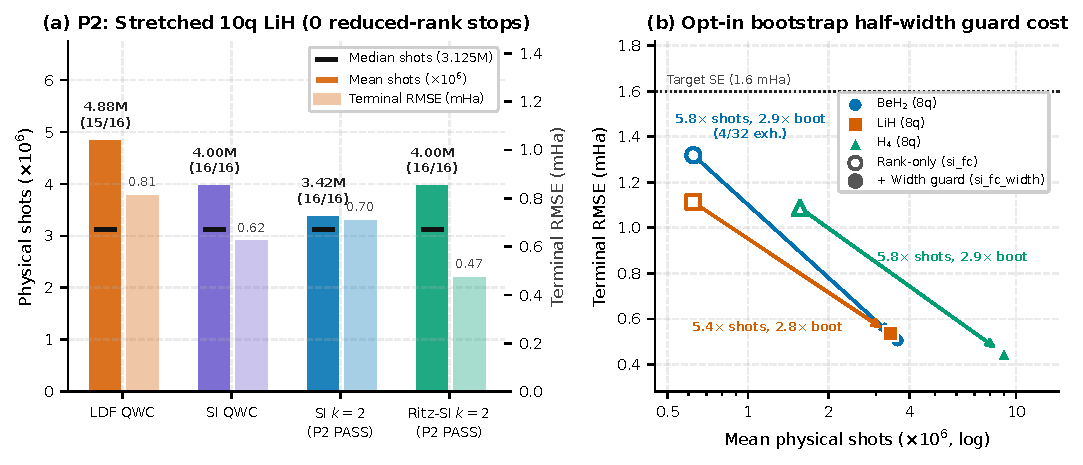
\includegraphics[width=\textwidth]{paper_assets/fig3_stretched_rank_and_width.pdf}
  \caption{(a)~Predeclared P2 transfer on the stretched ten-qubit LiH bank
  (\wpStretchedWords{} words, rank~4 straddling \(\tau_S=0.104\)): mean shots
  (solid bars, with true-stop count out of 16), median shots (black ticks), and
  terminal RMSE (hatched bars, right axis).  (b)~Shot-cost vs.\ RMSE shift from
  rank-only \texttt{si\_fc} (open symbols) to opt-in bootstrap half-width
  gating \texttt{si\_fc\_width} (filled symbols) across the three eight-qubit
  banks.}
  \label{fig:stretched_and_width}
\end{figure*}

\begin{table*}[t]
\centering
\caption{Predeclared P2 stretched ten-qubit LiH rank-stress transfer (Panel~A)
and opt-in bootstrap half-width guard overhead on eight-qubit banks (Panel~B).}
\label{tab:p2_and_width}
\tightcolumns
\begin{tabular}{l c c c c r c l}
\toprule
Arm / Bank & True stops & False (RR) & Med.\ / Mean (M) & Mean ratio (95\% CI) & RMSE (mHa) & 95\% boot (w / cond.) & Verdict / Boot cost \\
\midrule
% Auto-generated by paper_weighted_precision/make_tables.py. Do not edit.
\multicolumn{8}{l}{\textit{Panel A: Predeclared P2 --- Stretched 10-qubit LiH bank (10,341 words, rank 4, $\lambda_{\min}=0.10417$, $\tau_S=0.104$)}} \\
\midrule
\texttt{ldf\_qwc} & $15/16$ & $1$ ($0$) & $3.125$ / $4.883$ & baseline & $0.809$ & $16/16$ ($4.29$) & comparator \\
\texttt{si\_qwc} & $16/16$ & $0$ ($0$) & $3.125$ / $4.004$ & $0.820$ (ref.) & $0.620$ & $15/16$ ($3.17$) & comparator \\
\texttt{si\_k2} & $16/16$ & $0$ ($0$) & $3.125$ / $3.418$ & $0.700$ $[0.542, 0.927]$ & $0.705$ & $15/16$ ($3.21$) & \textbf{PASS} \\
\texttt{ritz\_si\_k2} & $16/16$ & $0$ ($0$) & $3.125$ / $4.004$ & $0.820$ $[0.593, 1.146]$ & $0.467$ & $16/16$ ($2.68$) & \textbf{PASS} \\
\midrule
\multicolumn{8}{l}{\textit{Panel B: Opt-in bootstrap half-width guard (\texttt{si\_fc\_width} vs.\ \texttt{si\_fc}) on 8-qubit banks}} \\
\midrule
BeH$_2$ (8q) & $28/32$ ($4$ exh.) & $0$ ($0$) & $3.906$ / $3.613$ & $5.781$ $[5.312, 6.133]$ & $0.506$ & $28/32$ ($28/28$ cond.) & $2.88\times$ boot \\
LiH (8q) & $31/32$ ($0$ exh.) & $1$ ($0$) & $3.906$ / $3.394$ & $5.430$ $[4.844, 5.898]$ & $0.535$ & $31/32$ ($31/32$) & $2.78\times$ boot \\
H$_4$ (8q) & $32/32$ ($0$ exh.) & $0$ ($0$) & $9.766$ / $9.033$ & $5.781$ $[5.312, 6.133]$ & $0.446$ & $31/32$ ($31/32$) & $2.88\times$ boot \\

\bottomrule
\end{tabular}
\end{table*}

Both weighted \(k=2\) arms pass P2 on \texttt{lih\_10q\_stretched}
(Table~\ref{tab:p2_and_width}, Panel~A; Fig.~\ref{fig:stretched_and_width}(a)).
With \(\lambda_{\min} = 0.10417\) sitting just \(1.7\times 10^{-4}\) above
\(\tau_S = 0.104\), \texttt{si\_k2} (\(490\) settings, \(\CZmax=5\), 2Q
depth~1) and \texttt{ritz\_si\_k2} (\(496\)--\(535\) settings, paid pilot
\(249{,}900\) shots) each achieve \(16/16\) true precision stops, \(0/16\)
false stops, and \(0\) reduced-rank stops.  Rank-margin confirmation pins the
median look at \(3.125\times 10^6\) shots for all four arms, while
\texttt{si\_k2} eliminates high-shot tail runs to reduce mean shots by
\wpStretchedSiKTwoSavePct{}\% versus \texttt{ldf\_qwc}
(\wpStretchedSiKTwoMeanM{}M vs.\ \wpStretchedLdfQwcMeanM{}M) and
\wpStretchedSiKTwoVsSiQwcPct{}\% versus \texttt{si\_qwc}.  Paid-pilot
\texttt{ritz\_si\_k2} reduces mean shots to \wpStretchedRitzRatioLdf{}\(\times\)
\texttt{ldf\_qwc} while achieving the lowest terminal RMSE
(\wpStretchedRitzRmse{} vs.\ \wpStretchedLdfRmse{}\,\(\mHa\)) and narrowest
95\% bootstrap interval (\wpStretchedRitzWidth{}\,\(\mHa\), \(16/16\)
coverage).

Table~\ref{tab:p2_and_width} (Panel~B) and
Fig.~\ref{fig:stretched_and_width}(b) quantify the opt-in bootstrap half-width
guard (\texttt{si\_fc\_width} vs.\ \texttt{si\_fc}).  Enforcing a \(1.6\,\mHa\)
six-look adjusted bootstrap half-width lowers terminal RMSE to
\wpWidthRmseMin{}--\wpWidthRmseMax{}\,\(\mHa\) and eliminates almost all
\(1\sigma\) false stops (\(0\)--\(1/32\)), at a cost of
\wpWidthMeanRatioMin{}\(\times\)--\wpWidthMeanRatioMax{}\(\times\) mean
physical shots and
\wpWidthBootRatioMin{}\(\times\)--\wpWidthBootRatioMax{}\(\times\) bootstrap
solves.  On BeH\(_2\)~(8q), \wpExhausted{}/32 attempts exhausted the
\(3.906\times 10^6\)-shot horizon despite actual errors of only
\wpWidthExhErrMin{}--\wpWidthExhErrMax{}\,\(\mHa\) because the Bonferroni-scaled
32-resample bootstrap half-width marginally exceeded \(1.6\,\mHa\)
(stop-conditional 95\% coverage \(28/28\), unconditional \(28/32\)).  This
confirms that bootstrap width gating should remain an explicit opt-in guard.

\subsection{P3: Gate-level noisy readout bias versus variance}
\label{sec:results_p3}

\begin{figure*}[t]
  \centering
  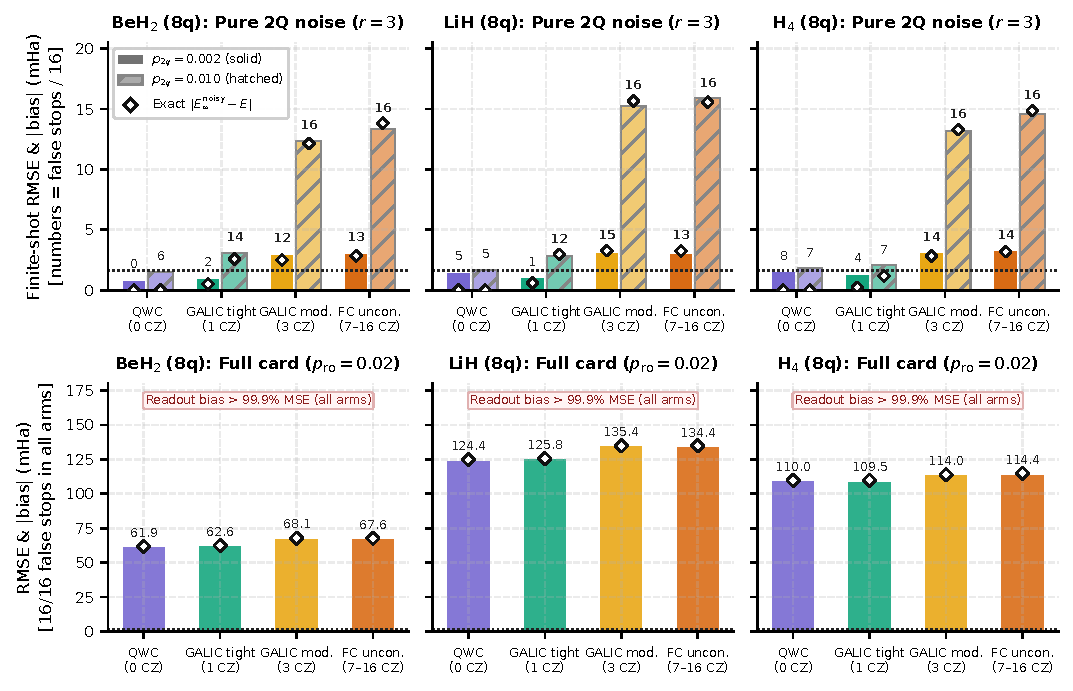
\includegraphics[width=\textwidth]{paper_assets/fig4_noisy_bias_variance.pdf}
  \caption{Part~B gate-level noisy readout evaluation across all 36 cells.
  Top row: pure two-qubit depolarizing noise (\(r_{\mathrm{route}}=3\)) at
  \(p_{2\mathrm{q}}=0.002\) (solid bars) and \(p_{2\mathrm{q}}=0.010\) (hatched
  bars); white diamonds mark exact infinite-shot bias
  \(|E_\infty^{\mathrm{noisy}} - E_{\mathrm{exact}}|\), numbers above bars give
  false precision stops out of 16, and dotted lines mark the \(1.6\,\mHa\)
  target.  Bottom row: full superconducting device card adding unmitigated
  readout bit-flip noise (\(p_{\mathrm{ro}}=0.02\)), where readout bias exceeds
  99.9\% of MSE across every arm including zero-2Q QWC.}
  \label{fig:noisy_bias}
\end{figure*}

All 576 Part~B acquisitions reached \texttt{target\_met} (\(0\) exhaustions,
\(0\) failures), demonstrating a central hazard of noisy adaptive stopping:
because two-qubit depolarizing channels shrink expectation values without
inflating shot-to-shot variance, an adaptive SE stop will stop confidently
around a biased energy.

Tight GALIC noise gating (\texttt{si\_fc\_galic\_tight}, \(\CZmax = 1\)) passes
all \wpPthreePassCount{}/\wpPthreeTotalCount{} pure-2Q P3 cells
(Fig.~\ref{fig:noisy_bias}, top row; full 36-cell ledger in
Table~\ref{tab:part_b_noisy}):
\begin{itemize}
  \item At \(p_{2\mathrm{q}}=0.002, r_{\mathrm{route}}=3\), unconstrained FC
    (\(\CZmax = 7\)--\(16\)) suffers \(+2.84\) to \(+3.25\,\mHa\) exact bias
    (\(82\)--\(88\%\) bias\(^2\) share) and
    \wpPtwoLowUncFalseMin{}--\wpPtwoLowUncFalseMax{}\(/16\) false precision
    stops.  Tight GALIC cuts exact bias by \(5.4\times\)--\wpBiasRedMax{}\(\times\)
    (to \(0.24\)--\(0.60\,\mHa\)), reduces RMSE by
    \wpRmseRedMin{}\(\times\)--\(3.0\times\), drops false stops to
    \wpPtwoLowTightFalseMin{}--\wpPtwoLowTightFalseMax{}\(/16\), and restores
    95\% unconditional bootstrap coverage to \(16/16\) on all three molecules.
    By contrast, moderate gating (\(\CZmax=3\)) already incurs \(+2.50\) to
    \(+3.27\,\mHa\) bias (\(12\)--\(15/16\) false stops), showing that
    \(\CZmax=3\) is too permissive for \(1.6\,\mHa\) precision at this error
    rate.
  \item At \(p_{2\mathrm{q}}=0.010, r_{\mathrm{route}}=3\), unconstrained FC
    collapses completely (\wpPtwoHighUncBiasMin{}--\wpPtwoHighUncBiasMax{}\,\(\mHa\)
    bias, \(16/16\) false stops, \(0/16\) coverage).  Tight GALIC slashes bias
    and RMSE by \wpBiasRedMin{}\(\times\)--\(12.7\times\) and
    \(4.3\times\)--\wpRmseRedMax{}\(\times\), respectively, and strictly lowers
    false stops on every molecule, but even a single routed CZ gate leaves
    \wpPtwoHighTightBiasMin{}--\wpPtwoHighTightBiasMax{}\,\(\mHa\) bias
    (\(7\)--\(14/16\) false stops), leaving zero-2Q \texttt{si\_qwc} as the
    only 2Q-unbiased choice at \(p_{2\mathrm{q}}=0.010, r_{\mathrm{route}}=3\).
  \item Under \texttt{sc\_card\_full} (\(p_{\mathrm{ro}}=0.02\);
    Fig.~\ref{fig:noisy_bias}, bottom row), unmitigated readout flip produces
    \(+\wpScFullBiasMin{}\) to \(+\wpScFullBiasMax{}\,\mHa\) exact bias
    (\(\ge 99.9\%\) bias\(^2\) share, \(16/16\) false stops, \(0/16\) coverage)
    across \emph{every} arm, including \texttt{si\_qwc}.  Two-qubit circuit
    gating therefore cannot substitute for readout error mitigation (REM); the
    two protections address orthogonal noise channels.
\end{itemize}

\section{Scope, Limitations, and Practical Guidance}
\label{sec:discussion}

Our findings yield a concrete engineering recipe for finite-shot subspace
measurement in \pkg{}:
\begin{enumerate}
  \item \textbf{Default to variance-weighted sorted insertion, never unweighted
    LDF.}  Weighted SI matches or beats LDF in \(9/9\) cells and delivers
    \(2.5\times\)--\wpPoneaSpeedupMax{}\(\times\) physical-shot savings in
    \(8/9\) cells at no extra circuit depth when \(k\) is fixed.
  \item \textbf{Always report empirical \(\Remp\) alongside \(\Rhat\), and test
    \(k=1\) and \(k=2\) before committing to FC.}  State-dependent covariance
    can invert the FC vs.\ QWC ordering (as on LiH), and \(k=2\) depth-1
    readouts already transfer cleanly to rank-stressed ten-qubit banks.
  \item \textbf{Use paid-pilot Ritz replanning when bank weights are diffuse,}
    billing every pilot shot explicitly to the total budget.
  \item \textbf{Pair GALIC two-qubit noise gating with dedicated readout error
    mitigation.}  At \(p_{2\mathrm{q}}=0.002, r_{\mathrm{route}}=3\),
    \(\CZmax=1\) preserves sub-mHa bias; at \(p_{2\mathrm{q}}=0.010,
    r_{\mathrm{route}}=3\), fall back to QWC (\(\CZmax=0\)) unless two-qubit
    error mitigation is active.
  \item \textbf{Keep rank/margin confirmation as the default stopping guard and
    bootstrap half-width gating as opt-in} when strict \(1\sigma\) error
    suppression justifies a \(5\times\)--\(6\times\) shot multiplier.
\end{enumerate}

\emph{Explicit non-claims.}  All experiments use ideal statevector or
explicit depolarizing/bit-flip gate-level simulation on fixed small molecular
banks (8--10 qubits, 3--4 basis directions).  Targets are the declared
fixed-bank projected energies rather than full-CI chemical accuracy.  We do not
claim hardware performance, asymptotic scaling, quantum advantage, or
finite-sample/anytime-valid interval guarantees.  The single failed P1a cell on
LiH (\(k=8\)) and the readout-dominated failure of all arms under
\texttt{sc\_card\_full} are retained as first-class experimental outcomes.

\section{Reproducibility and Provenance}
\label{sec:reproducibility}

The study enforces a strict two-commit separation in Git: the result-free
declaration, runner, checker, and analysis code were merged at commit
\texttt{\wpDeclCommitFull}, and the compressed evaluation artifact
\texttt{docs/restart/weighted\_precision\_results.json.gz} was committed only
in a descendant commit after clean-worktree execution under Python~\wpPythonVer,
NumPy~\wpNumpyVer, SciPy~\wpScipyVer, and single-threaded BLAS.  Routine CI
runs \texttt{benchmarks/check\_weighted\_precision.py --verify-history} under
that exact declared runtime, re-auditing Git ancestry, source digests, all
\wpNoisyAnchorCount{} independent noisy anchors, and all \wpTotalAcq{}
acquisition rows.  Every table, macro, and figure in this manuscript is
generated programmatically from those frozen records and audited by
\texttt{paper\_weighted\_precision/check\_manuscript.py}.

\appendix
\section{Complete Experimental Ledgers}
\label{app:ledgers}

Tables~\ref{tab:part_a_full} and~\ref{tab:part_b_noisy} report the complete
28-cell Part~A and 36-cell Part~B outcomes underlying Figs.~\ref{fig:shot_savings}--\ref{fig:noisy_bias}
and Tables~\ref{tab:p1_verdicts}--\ref{tab:p2_and_width}.

\begin{table*}[p]
\centering
\caption{Complete Part~A ideal-shot ledger across all 28 \texttt{(case, arm)}
cells (\wpPartAAcq{} acquisitions).  Unconditional coverage counts eligible
\texttt{target\_met} stops over all declared attempts; parenthesized widths
are median interval widths in mHa among stops.  Stop-conditional coverage
equals unconditional coverage in every cell except BeH\(_2\)~(8q)
\texttt{si\_fc\_width} (\(28/28\) at 95\%, \(26/28\) at 68\%, with 4 schedule
exhaustions).}
\label{tab:part_a_full}
\compactcolumns
\scriptsize
\begin{tabular}{l l c c c r r c c c r}
\toprule
Bank & Arm & Stops (exh.) & True/False & Med./Mean (M) & Dev.\ (s) & RMSE & 95\% boot (w) & 95\% delta (w) & 68\% boot (w) & \(\Remp/\Rhat\) \\
\midrule
% Auto-generated by paper_weighted_precision/make_tables.py. Do not edit.
BeH$_2$ (8q) & \texttt{ldf\_qwc} & $32/32$ & $25/7$ & $1.562$ / $1.562$ & $15.75$ & $1.484$ & $30/32$ ($7.11$) & $30/32$ ($6.96$) & $29/32$ ($5.21$) & $30/32$ ($5.10$) & $0.272$ \\
 & \texttt{si\_qwc} & $32/32$ & $30/2$ & $0.625$ / $0.625$ & $6.30$ & $0.899$ & $32/32$ ($4.72$) & $32/32$ ($5.43$) & $30/32$ ($3.46$) & $32/32$ ($3.98$) & $0.531$ \\
 & \texttt{ldf\_k2} & $32/32$ & $26/6$ & $1.562$ / $1.562$ & $16.25$ & $1.239$ & $31/32$ ($6.26$) & $32/32$ ($6.46$) & $31/32$ ($4.59$) & $31/32$ ($4.73$) & $0.217$ \\
 & \texttt{si\_k2} & $32/32$ & $24/8$ & $0.250$ / $0.273$ & $2.58$ & $1.362$ & $32/32$ ($7.54$) & $32/32$ ($7.91$) & $32/32$ ($5.53$) & $32/32$ ($5.79$) & $0.386$ \\
 & \texttt{ldf\_fc} & $32/32$ & $28/4$ & $1.562$ / $1.562$ & $17.26$ & $1.075$ & $32/32$ ($5.11$) & $32/32$ ($5.49$) & $30/32$ ($3.74$) & $30/32$ ($4.02$) & $0.171$ \\
 & \texttt{si\_fc} & $32/32$ & $26/6$ & $0.625$ / $0.625$ & $6.89$ & $1.319$ & $31/32$ ($6.92$) & $31/32$ ($7.15$) & $30/32$ ($5.06$) & $31/32$ ($5.24$) & $0.209$ \\
 & \texttt{ritz\_si\_fc} & $32/32$ & $25/7$ & $0.250$ / $0.250$ & $2.70$ & $1.260$ & $32/32$ ($5.87$) & $32/32$ ($6.48$) & $28/32$ ($4.30$) & $31/32$ ($4.74$) & $0.348$ \\
 & \texttt{si\_fc\_width} & $28/32$ ($4$) & $28/0$ & $3.906$ / $3.613$ & $43.05$ & $0.506$ & $28/32$ ($2.63$) & $28/32$ ($2.83$) & $26/32$ ($1.92$) & $27/32$ ($2.07$) & $0.208$ \\
\midrule
LiH (8q) & \texttt{ldf\_qwc} & $32/32$ & $26/6$ & $3.906$ / $3.394$ & $39.43$ & $1.352$ & $30/32$ ($5.53$) & $31/32$ ($5.77$) & $29/32$ ($4.05$) & $30/32$ ($4.22$) & $1.339$ \\
 & \texttt{si\_qwc} & $32/32$ & $25/7$ & $0.250$ / $0.250$ & $2.52$ & $1.511$ & $31/32$ ($7.79$) & $31/32$ ($8.13$) & $30/32$ ($5.70$) & $30/32$ ($5.95$) & $3.799$ \\
 & \texttt{ldf\_k2} & $32/32$ & $23/9$ & $1.562$ / $1.782$ & $16.18$ & $1.571$ & $31/32$ ($7.76$) & $32/32$ ($7.91$) & $28/32$ ($5.69$) & $29/32$ ($5.79$) & $1.367$ \\
 & \texttt{si\_k2} & $32/32$ & $25/7$ & $0.250$ / $0.320$ & $2.58$ & $1.450$ & $32/32$ ($7.38$) & $32/32$ ($8.17$) & $30/32$ ($5.41$) & $28/32$ ($5.98$) & $2.799$ \\
 & \texttt{ldf\_fc} & $32/32$ & $28/4$ & $0.625$ / $0.625$ & $6.87$ & $1.167$ & $31/32$ ($5.79$) & $32/32$ ($6.36$) & $30/32$ ($4.24$) & $29/32$ ($4.66$) & $1.501$ \\
 & \texttt{si\_fc} & $32/32$ & $26/6$ & $0.625$ / $0.625$ & $6.87$ & $1.113$ & $32/32$ ($5.89$) & $32/32$ ($6.42$) & $30/32$ ($4.32$) & $32/32$ ($4.70$) & $1.397$ \\
 & \texttt{ritz\_si\_fc} & $32/32$ & $27/5$ & $0.625$ / $0.602$ & $6.78$ & $1.189$ & $32/32$ ($5.90$) & $32/32$ ($5.76$) & $29/32$ ($4.32$) & $30/32$ ($4.22$) & $1.628$ \\
 & \texttt{si\_fc\_width} & $32/32$ & $31/1$ & $3.906$ / $3.394$ & $42.92$ & $0.535$ & $31/32$ ($2.49$) & $32/32$ ($2.53$) & $30/32$ ($1.83$) & $31/32$ ($1.85$) & $1.396$ \\
\midrule
H$_4$ (8q) & \texttt{ldf\_qwc} & $32/32$ & $25/7$ & $9.766$ / $9.766$ & $98.58$ & $1.341$ & $30/32$ ($5.97$) & $31/32$ ($6.21$) & $29/32$ ($4.37$) & $29/32$ ($4.55$) & $0.844$ \\
 & \texttt{si\_qwc} & $32/32$ & $21/11$ & $3.906$ / $3.906$ & $39.40$ & $1.482$ & $32/32$ ($7.06$) & $32/32$ ($7.90$) & $28/32$ ($5.17$) & $29/32$ ($5.79$) & $0.480$ \\
 & \texttt{ldf\_k2} & $32/32$ & $29/3$ & $9.766$ / $9.766$ & $101.11$ & $1.044$ & $31/32$ ($5.51$) & $32/32$ ($5.73$) & $30/32$ ($4.03$) & $30/32$ ($4.20$) & $0.669$ \\
 & \texttt{si\_k2} & $32/32$ & $27/5$ & $3.906$ / $3.906$ & $40.29$ & $1.443$ & $30/32$ ($6.88$) & $31/32$ ($7.62$) & $29/32$ ($5.04$) & $29/32$ ($5.58$) & $0.394$ \\
 & \texttt{ldf\_fc} & $32/32$ & $30/2$ & $3.906$ / $3.906$ & $44.18$ & $0.992$ & $32/32$ ($5.50$) & $32/32$ ($5.83$) & $31/32$ ($4.03$) & $31/32$ ($4.27$) & $0.468$ \\
 & \texttt{si\_fc} & $32/32$ & $27/5$ & $1.562$ / $1.562$ & $17.27$ & $1.088$ & $32/32$ ($6.42$) & $32/32$ ($6.62$) & $32/32$ ($4.70$) & $32/32$ ($4.85$) & $0.512$ \\
 & \texttt{ritz\_si\_fc} & $32/32$ & $26/6$ & $1.562$ / $1.562$ & $17.20$ & $1.133$ & $32/32$ ($6.13$) & $32/32$ ($6.18$) & $31/32$ ($4.49$) & $31/32$ ($4.53$) & $0.547$ \\
 & \texttt{si\_fc\_width} & $32/32$ & $32/0$ & $9.766$ / $9.033$ & $107.82$ & $0.446$ & $31/32$ ($2.62$) & $32/32$ ($2.61$) & $30/32$ ($1.92$) & $30/32$ ($1.92$) & $0.511$ \\
\midrule
LiH (10q, str.) & \texttt{ldf\_qwc} & $16/16$ & $15/1$ & $3.125$ / $4.883$ & $37.80$ & $0.809$ & $16/16$ ($4.29$) & $16/16$ ($5.43$) & $16/16$ ($3.08$) & $16/16$ ($3.90$) & $0.792$ \\
 & \texttt{si\_qwc} & $16/16$ & $16/0$ & $3.125$ / $4.004$ & $37.78$ & $0.620$ & $15/16$ ($3.17$) & $16/16$ ($3.70$) & $14/16$ ($2.28$) & $16/16$ ($2.66$) & $0.391$ \\
 & \texttt{si\_k2} & $16/16$ & $16/0$ & $3.125$ / $3.418$ & $38.72$ & $0.705$ & $15/16$ ($3.21$) & $16/16$ ($3.93$) & $14/16$ ($2.31$) & $16/16$ ($2.83$) & $0.325$ \\
 & \texttt{ritz\_si\_k2} & $16/16$ & $16/0$ & $3.125$ / $4.004$ & $38.63$ & $0.467$ & $16/16$ ($2.68$) & $16/16$ ($3.11$) & $15/16$ ($1.93$) & $15/16$ ($2.23$) & $0.330$ \\

\bottomrule
\end{tabular}
\end{table*}

\begin{table*}[p]
\centering
\caption{Complete Part~B gate-level noisy readout ledger across all 36
\texttt{(case, regime, arm)} cells (\wpPartBAcq{} acquisitions; all 576 reached
\texttt{target\_met} with \(0\) reduced-rank stops).  Columns show setting
count (\(\CZmax\)), true/false \(1.6\,\mHa\) stops, exact infinite-shot noisy
bias \(E_\infty^{\mathrm{noisy}} - E_{\mathrm{exact}}\), finite-shot empirical
bias \(\pm\) std, RMSE, bias\(^2\) share of MSE, unconditional 95\% bootstrap
coverage, and P3 verdict.}
\label{tab:part_b_noisy}
\compactcolumns
\scriptsize
\begin{tabular}{l l l c c r c r r c l}
\toprule
Bank & Regime & Arm & Set.\ (\(\CZmax\)) & T/F & \(E_\infty\) bias & Emp.\ bias \(\pm\) std & RMSE & Bias\(^2\) & 95\% boot & P3 \\
\midrule
% Auto-generated by paper_weighted_precision/make_tables.py. Do not edit.
BeH$_2$ (8q) & \texttt{depol2q\_p002} & \texttt{si\_qwc} & $312$ ($0$) & $16/0$ & $0.625$ & $0.000$ & $-0.344 \pm 0.804$ & $0.874$ & $15.5\%$ & $16/16$ &  \\
 &  & \texttt{si\_fc\_unc} & $14$ ($7$) & $3/13$ & $0.625$ & $+2.841$ & $+2.828 \pm 1.307$ & $3.116$ & $82.4\%$ & $11/16$ &  \\
 &  & \texttt{si\_fc\_tight} & $307$ ($1$) & $14/2$ & $0.625$ & $-0.520$ & $-0.608 \pm 0.856$ & $1.050$ & $33.5\%$ & $16/16$ & \textbf{PASS} \\
 &  & \texttt{si\_fc\_mod} & $150$ ($3$) & $4/12$ & $0.625$ & $+2.498$ & $+2.673 \pm 1.384$ & $3.010$ & $78.9\%$ & $12/16$ &  \\
\midrule
BeH$_2$ (8q) & \texttt{depol2q\_p010} & \texttt{si\_qwc} & $312$ ($0$) & $10/6$ & $0.625$ & $0.000$ & $-0.412 \pm 1.484$ & $1.540$ & $7.2\%$ & $13/16$ &  \\
 &  & \texttt{si\_fc\_unc} & $14$ ($7$) & $0/16$ & $0.625$ & $+13.820$ & $+13.282 \pm 0.966$ & $13.317$ & $99.5\%$ & $0/16$ &  \\
 &  & \texttt{si\_fc\_tight} & $307$ ($1$) & $2/14$ & $0.625$ & $-2.578$ & $-2.946 \pm 0.979$ & $3.104$ & $90.1\%$ & $7/16$ & \textbf{PASS} \\
 &  & \texttt{si\_fc\_mod} & $150$ ($3$) & $0/16$ & $0.625$ & $+12.147$ & $+12.302 \pm 1.223$ & $12.362$ & $99.0\%$ & $0/16$ &  \\
\midrule
BeH$_2$ (8q) & \texttt{sc\_card\_full} & \texttt{si\_qwc} & $312$ ($0$) & $0/16$ & $0.625$ & $+61.783$ & $+61.843 \pm 1.215$ & $61.855$ & $100.0\%$ & $0/16$ & diag. \\
 &  & \texttt{si\_fc\_unc} & $14$ ($7$) & $0/16$ & $0.625$ & $+67.753$ & $+67.621 \pm 1.700$ & $67.643$ & $99.9\%$ & $0/16$ &  \\
 &  & \texttt{si\_fc\_tight} & $307$ ($1$) & $0/16$ & $0.625$ & $+62.414$ & $+62.592 \pm 0.949$ & $62.599$ & $100.0\%$ & $0/16$ &  \\
 &  & \texttt{si\_fc\_mod} & $150$ ($3$) & $0/16$ & $0.625$ & $+67.857$ & $+68.097 \pm 1.307$ & $68.110$ & $100.0\%$ & $0/16$ &  \\
\midrule
LiH (8q) & \texttt{depol2q\_p002} & \texttt{si\_qwc} & $768$ ($0$) & $11/5$ & $0.273$ & $0.000$ & $+0.322 \pm 1.510$ & $1.544$ & $4.4\%$ & $14/16$ &  \\
 &  & \texttt{si\_fc\_unc} & $59$ ($12$) & $3/13$ & $0.625$ & $+3.250$ & $+2.792 \pm 1.208$ & $3.042$ & $84.2\%$ & $11/16$ &  \\
 &  & \texttt{si\_fc\_tight} & $720$ ($1$) & $15/1$ & $0.602$ & $-0.598$ & $-0.464 \pm 0.950$ & $1.057$ & $19.2\%$ & $16/16$ & \textbf{PASS} \\
 &  & \texttt{si\_fc\_mod} & $282$ ($3$) & $1/15$ & $0.625$ & $+3.274$ & $+3.021 \pm 0.866$ & $3.143$ & $92.4\%$ & $11/16$ &  \\
\midrule
LiH (8q) & \texttt{depol2q\_p010} & \texttt{si\_qwc} & $768$ ($0$) & $11/5$ & $0.273$ & $0.000$ & $+0.230 \pm 1.684$ & $1.699$ & $1.8\%$ & $16/16$ &  \\
 &  & \texttt{si\_fc\_unc} & $59$ ($12$) & $0/16$ & $0.625$ & $+15.555$ & $+15.798 \pm 1.558$ & $15.874$ & $99.0\%$ & $0/16$ &  \\
 &  & \texttt{si\_fc\_tight} & $720$ ($1$) & $4/12$ & $0.602$ & $-2.967$ & $-2.566 \pm 1.274$ & $2.865$ & $80.2\%$ & $8/16$ & \textbf{PASS} \\
 &  & \texttt{si\_fc\_mod} & $282$ ($3$) & $0/16$ & $0.625$ & $+15.663$ & $+15.215 \pm 1.007$ & $15.248$ & $99.6\%$ & $0/16$ &  \\
\midrule
LiH (8q) & \texttt{sc\_card\_full} & \texttt{si\_qwc} & $768$ ($0$) & $0/16$ & $0.625$ & $+124.854$ & $+124.412 \pm 1.136$ & $124.417$ & $100.0\%$ & $0/16$ & diag. \\
 &  & \texttt{si\_fc\_unc} & $59$ ($12$) & $0/16$ & $1.562$ & $+134.882$ & $+134.365 \pm 1.180$ & $134.371$ & $100.0\%$ & $0/16$ &  \\
 &  & \texttt{si\_fc\_tight} & $720$ ($1$) & $0/16$ & $0.625$ & $+125.539$ & $+125.830 \pm 1.725$ & $125.841$ & $100.0\%$ & $0/16$ &  \\
 &  & \texttt{si\_fc\_mod} & $282$ ($3$) & $0/16$ & $1.562$ & $+134.856$ & $+135.357 \pm 1.578$ & $135.366$ & $100.0\%$ & $0/16$ &  \\
\midrule
H$_4$ (8q) & \texttt{depol2q\_p002} & \texttt{si\_qwc} & $794$ ($0$) & $8/8$ & $3.906$ & $0.000$ & $+0.207 \pm 1.541$ & $1.555$ & $1.8\%$ & $16/16$ &  \\
 &  & \texttt{si\_fc\_unc} & $61$ ($16$) & $2/14$ & $1.562$ & $+3.187$ & $+3.093 \pm 1.123$ & $3.290$ & $88.4\%$ & $8/16$ &  \\
 &  & \texttt{si\_fc\_tight} & $745$ ($1$) & $12/4$ & $3.906$ & $+0.237$ & $+0.702 \pm 1.167$ & $1.362$ & $26.6\%$ & $16/16$ & \textbf{PASS} \\
 &  & \texttt{si\_fc\_mod} & $297$ ($3$) & $2/14$ & $1.562$ & $+2.827$ & $+2.928 \pm 1.164$ & $3.151$ & $86.4\%$ & $11/16$ &  \\
\midrule
H$_4$ (8q) & \texttt{depol2q\_p010} & \texttt{si\_qwc} & $794$ ($0$) & $9/7$ & $3.906$ & $0.000$ & $+0.324 \pm 1.775$ & $1.804$ & $3.2\%$ & $14/16$ &  \\
 &  & \texttt{si\_fc\_unc} & $61$ ($16$) & $0/16$ & $1.562$ & $+14.853$ & $+14.587 \pm 0.963$ & $14.619$ & $99.6\%$ & $0/16$ &  \\
 &  & \texttt{si\_fc\_tight} & $745$ ($1$) & $9/7$ & $3.906$ & $+1.172$ & $+1.548 \pm 1.348$ & $2.052$ & $56.9\%$ & $13/16$ & \textbf{PASS} \\
 &  & \texttt{si\_fc\_mod} & $297$ ($3$) & $0/16$ & $1.562$ & $+13.285$ & $+13.055 \pm 1.790$ & $13.177$ & $98.2\%$ & $0/16$ &  \\
\midrule
H$_4$ (8q) & \texttt{sc\_card\_full} & \texttt{si\_qwc} & $794$ ($0$) & $0/16$ & $3.906$ & $+109.736$ & $+110.032 \pm 1.321$ & $110.040$ & $100.0\%$ & $0/16$ & diag. \\
 &  & \texttt{si\_fc\_unc} & $61$ ($16$) & $0/16$ & $1.562$ & $+114.980$ & $+114.376 \pm 1.301$ & $114.384$ & $100.0\%$ & $0/16$ &  \\
 &  & \texttt{si\_fc\_tight} & $745$ ($1$) & $0/16$ & $3.906$ & $+109.806$ & $+109.439 \pm 1.626$ & $109.451$ & $100.0\%$ & $0/16$ &  \\
 &  & \texttt{si\_fc\_mod} & $297$ ($3$) & $0/16$ & $3.906$ & $+113.799$ & $+114.035 \pm 0.794$ & $114.037$ & $100.0\%$ & $0/16$ &  \\

\bottomrule
\end{tabular}
\end{table*}

\bibliographystyle{apsrev4-2}
\bibliography{references}

\end{document}
